\documentclass{beamer}
\usetheme{Montpellier}
\usecolortheme{dolphin}

%\usepackage{graphicx} %For jpg figure inclusion
%\usepackage{times} %For typeface
%\usepackage{epsfig}
\usepackage{color} %For Comments
\usepackage{beamerthemeshadow} %Paul and Lemmon put this in, take out if you want
%\usepackage[all]{xy}
%\usepackage{float}
%\usepackage{subfigure} 
%\usepackage{hyperref}
%\usepackage{url}
%\usepackage{parskip}
%\usepackage{multirow}

%% Elena's favorite green (thanks, Fernando!)
\definecolor{ForestGreen}{RGB}{34,139,34}
% Uncomment this if you want to show work-in-progress comments
\newcommand{\comment}[1]{{\bf \tt  {#1}}}
% Uncomment this if you don't want to show comments
%\newcommand{\comment}[1]{}
\newcommand{\emcomment}[1]{\textcolor{ForestGreen}{\comment{Elena: {#1}}}}
%%%%%%%%%%%%%%%%%%%%%%%%%%%%%%%%%%%%%%%%%%

\begin{document}
\title{Discussion about inclusiveness in CSci}
\author{UMM CSci}
\date{October 5, 2015}

\begin{frame}
\maketitle
\end{frame}

\begin{frame}
\frametitle{Why talk about inclusiveness?}
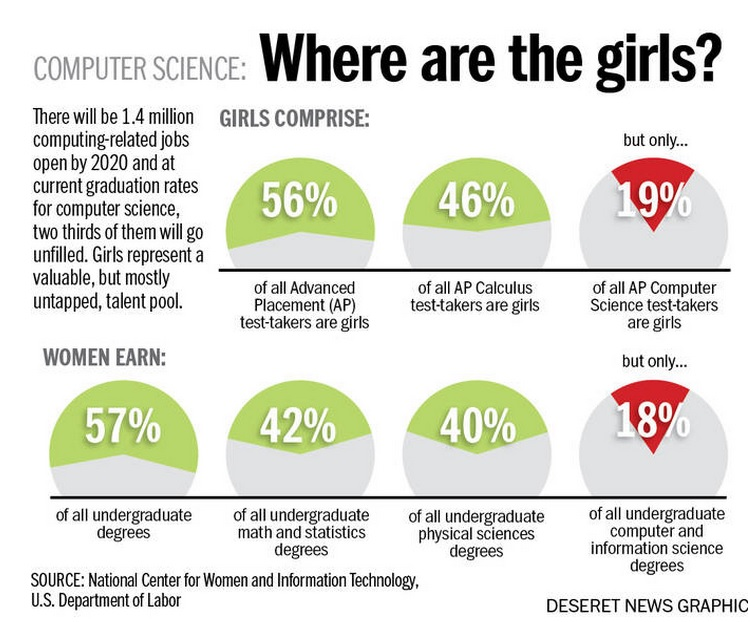
\includegraphics[scale=0.5]{Stats.jpg}
\end{frame}

\begin{frame}
\frametitle{Two videos}
What is the issue? 

{\it 
\href{https://www.youtube.com/watch?v=fQyCBTDproE}{The Underrepresentation of Women in STEM, by Chelsea Ziadle}}

A story of a woman engineer:

{\it
\href{https://www.youtube.com/watch?v=FEeTLopLkEo}{Inspiring the next generation of female engineers: Debbie Sterling at TEDxPSU}}

Similar problems are faced by ethnic minorities or anyone else who doesn't look like a stereotypical  person working in a tech field. 
\end{frame}

\begin{frame}
\frametitle{\#IlookLikeAnEngineer twitter campaign}
Isis Wenger, a platform engineer at OneLogin, was photographed for a recruiting ad: 
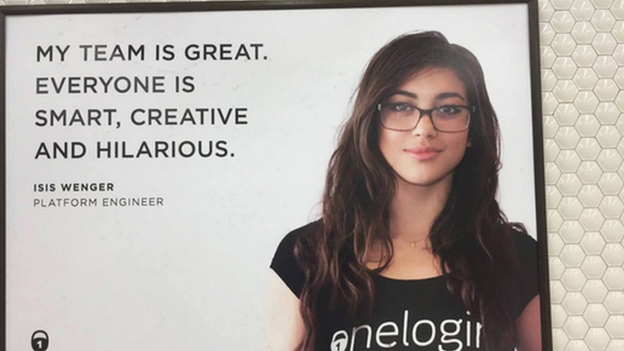
\includegraphics[scale=0.5]{engineer.png}

Comments on social media: people thought she was a photo model, not an engineer, and the quote was made up. 
\end{frame}

\begin{frame}
\frametitle{\#IlookLikeAnEngineer twitter campaign}
{\it \href{https://medium.com/the-coffeelicious/you-may-have-seen-my-face-on-bart-8b9561003e0f}{Isis Wenger's blog post}} lists her experiences, including male colleagues throwing dollar bills at her in the office, or a colleague messaging her seeking to be ``friends with benefits''. She says it doesn't indicate that they are bad people, just that people don't know how their ``playful'' behavior affects those it's directed at. 

\vspace{0.2in}

\#IlookLikeAnEngineer twitter campaign in response: {\it \href{http://www.bbc.com/news/blogs-trending-33783007}{hundreds of engineers who may not look stereotypical posting their pictures}}.  

\vspace{0.2in}

{\it \href{https://twitter.com/hashtag/ILookLikeanengineer}{https://twitter.com/hashtag/ILookLikeanengineer}}

\end{frame}

\begin{frame}
\frametitle{Well-meaning attempts to get underrepresented groups into tech.....}
South African pen manufacturing company Bic posted this ad on its Facebook page to celebrate national women's day:

\includegraphics[scale=0.15]{thinklikeaman.jpg}

{\tiny \href{http://www.theguardian.com/society/2015/aug/11/look-like-a-girl-think-like-a-man-bic-outrage-south-africa-womens-day}{http://www.theguardian.com/society/2015/aug/11/look-like-a-girl-think-like-a-man-bic-outrage-south-africa-womens-day}}
\end{frame}

\begin{frame}
\frametitle{Study shows gender bias in math grading}
\begin{itemize}
\item {\it \href{http://www.slate.com/blogs/xx_factor/2015/02/10/teacher_bias_in_math_new_study_finds_teachers_grade_boys_more_generously.html}{A study by Victor Lavy of the University of Warwick in England and Edith Sand of Tel Aviv University (2015)}}.
\item Three groups of Israeli students, grade 6 to end of high school.
\item 2 math exams: one graded by outsiders not given the students' names, the other by teachers who knew their names.
\item In the exam graded anonymously, girls outperformed boys.
\item In  the exam graded by teachers who knew their names, boys outperformed girls.
\item There was no similar effect in other areas (e.g. language). 
\item Studies show that belief in one's abilities greatly increases performance. 
\item Since girls aren't expected, or encouraged, to do well in math, they perform worse or drop out.
\item The teachers in the study were women.
\end{itemize}
\end{frame}

\begin{frame}
\frametitle{Starting points for group discussion}
\begin{itemize}
\item Why is diversity so important? 
\begin{itemize}
\item What problems arise due to lack of diversity in STEM fields?
\item How can our experiences (or lack of experience) with diversity influence us?
\end{itemize}
\item Have you encountered messages designed for women and minorities that imply that they aren’t good at math or science?
\item In what instances have media tried to promote diversity in an ineffective way?
\item How do you feel diversity has affected your academic experience?
\item How can we promote diversity and inclusiveness in the Computer Science program here at Morris?
\begin{itemize}
\item What are we doing well? 
\item What can be improved?
\end{itemize}
\end{itemize}
\end{frame}

\begin{frame}
\frametitle{Resources}
\begin{itemize}
{\tiny 
\item The Underrepresentation of Women in STEM, by Chelsea Ziadle: \href{https://www.youtube.com/watch?v=fQyCBTDproE}{https://www.youtube.com/watch?v=fQyCBTDproE}
\item Inspiring the next generation of female engineers: Debbie Sterling at TEDxPSU \href{https://www.youtube.com/watch?v=FEeTLopLkEo}{https://www.youtube.com/watch?v=FEeTLopLkEo}
\item \#IlookLikeAnEngineer twitter campaign:  Isis Wenger blog post: \href{https://medium.com/the-coffeelicious/you-may-have-seen-my-face-on-bart-8b9561003e0f}{https://medium.com/the-coffeelicious/you-may-have-seen-my-face-on-bart-8b9561003e0f}, the BBC article about it: \href{http://www.bbc.com/news/blogs-trending-33783007}{http://www.bbc.com/news/blogs-trending-33783007}
\item Bic ad story: \href{http://www.theguardian.com/society/2015/aug/11/look-like-a-girl-think-like-a-man-bic-outrage-south-africa-womens-day}{http://www.theguardian.com/society/2015/aug/11/look-like-a-girl-think-like-a-man-bic-outrage-south-africa-womens-day}
\item The math grading bias study: \href{http://www.slate.com/blogs/xx_factor/2015/02/10/teacher_bias_in_math_new_study_finds_teachers_grade_boys_more_generously.html}{http://www.slate.com/blogs/xx$\_$factor/2015/02/10/teacher$\_$bias$\_$in$\_$math$\_$new$\_$study$\_$finds$\_$teachers$\_$grade$\_$boys$\_$more$\_$generously.html}
\item Barbie book about programming story (was brought up in one of the discussion groups): \href{http://www.dailydot.com/geek/barbie-engineer-book-girls-game-developers/}{http://www.dailydot.com/geek/barbie-engineer-book-girls-game-developers/}
}
\end{itemize}
\end{frame}



\end{document}